\documentclass[12pt]{article}
\usepackage{geometry}
\geometry{a4paper, bottom=40mm, top=40mm, left=25mm, right=25mm}
\usepackage{pdfpages}
\usepackage{fancyhdr}
\pagestyle{fancy}
\setlength{\parindent}{0cm}
\setlength{\headheight}{14pt}
\usepackage{parskip}
\usepackage{tocloft}
\usepackage[export]{adjustbox}
\usepackage{float}
\usepackage{subfig}
\usepackage{graphicx}
\graphicspath{{../figures}}
\usepackage{amsmath,blkarray,booktabs,bigstrut, amssymb}
\usepackage{pythonhighlight}
\usepackage{outlines}
\usepackage[hidelinks]{hyperref}
\usepackage[backend=biber, style=ieee]{biblatex}
\addbibresource{references.bib}
% \nocite{*}
\usepackage{url}
\setcounter{biburllcpenalty}{7000}
\setcounter{biburlucpenalty}{8000}
\widowpenalty10000
\clubpenalty10000
\setcounter{secnumdepth}{0}


\begin{document}

\newgeometry{top=20mm}
\begin{titlepage}
    \begin{center}
      \begin{figure}
        
\includegraphics[right]{logo.png}
      \end{figure}
      \vspace*{1cm}
      \textsc{\large ENEL373: Digital Electronics and Devices}\\[0.5cm]
      \textsc{\Large University of Canterbury}\\[3.5cm]
      \linespread{1}
      {\Huge\bfseries This is an Awesome Title \\[0.3cm] for Our First Report} \\
      \vspace*{2cm}
      {\Huge Philip Brand \textit{\Large(15776928)}\\\par}
      % ADD YOUR NAME AND STUDENT ID HERE
      \vspace*{3cm}
      {\LARGE \today}
    \end{center}
  \end{titlepage}
\restoregeometry

\fancyhead{}
\fancyhead[L]{\small{ENEL373 - Reaction Timer Project}}
\fancyhead[R]{\small{\today}}

\pagenumbering{roman}

\addcontentsline{toc}{section}{Abstract}
\section*{Abstract}

Not sure if we need an abstract

\newpage

\renewcommand{\baselinestretch}{1.3}\normalsize
\setlength{\cftbeforesecskip}{0.3em}
\renewcommand{\cftsecleader}{\cftdotfill{\cftdotsep}}
\addcontentsline{toc}{section}{Contents}
\tableofcontents\thispagestyle{fancy}
\renewcommand{\baselinestretch}{1}\normalsize

\newpage
\pagenumbering{arabic}

\section{Introduction}
% Outline (in your own words) the project requirements and what you achieved

Here is how we include a figure in the report. Figure \ref{fig:example} shows an example of a figure. A figure.

\begin{figure}[H]
  \centering
  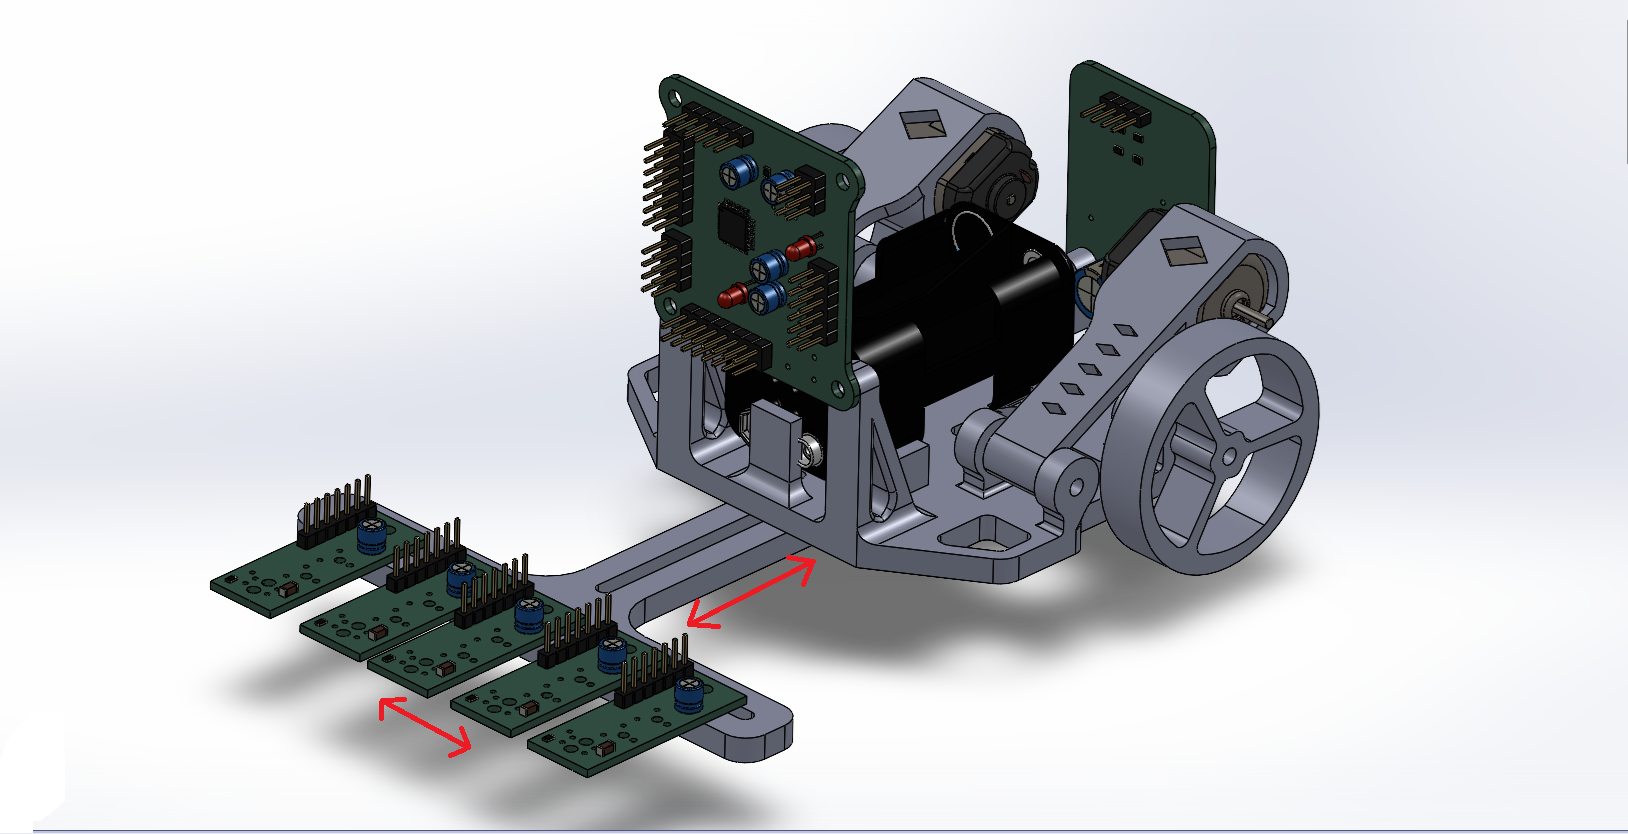
\includegraphics[width=0.8\textwidth]{example.png}
  \caption{This is an example of a figure.}
  \label{fig:example}
\end{figure}

\newpage

\section{Design Summary}
% Summarise your design.

\newpage

\section{Design Details}
% (~2 pages): Describe the methods your group used to implement your FPGA design. Justify your final design. Support your descriptions and justifications with specific, explicit references to your VHDL source code in the appendix. VHDL descriptions could, for example, include an RTL description.

\newpage

\section{Module Testing}
% A brief section describing how you tested a significant module. Include at least one testbench and associated waveforms that demonstrate the functionality of a module in the report appendix.

\newpage

\section{Conclusions}
% Highlight any problems you encountered and how you solved them. Also discuss what you learned and give suggestions on how the project could be improved


\newpage
% There is no need to include a full code listing in your report as your code will be submitted via eng-git. However, reference to a code snippet in an appendix is quite appropriate. Formal citations to books, web articles, open source VHDL code and other sources should be listed in a reference section that uses the IEEE style and format.


\printbibliography

\appendix


\end{document}
